% ============================================================
% ANHANG B – Diagramme in A4 Querformat (Grossansicht)
% ============================================================
% Voraussetzung im Preamble: \usepackage{pdflscape}
% ============================================================

\section{Anhang~B: Diagramme in A4\,Quer -- Grossansicht}
\label{sec:anhang-diagramme}

\begin{hinweis}[Hinweis zur Lesbarkeit]
Die folgenden Diagramme sind identisch mit den im Fliesstext eingebetteten
Abbildungen, werden hier jedoch auf A4-Querformat dargestellt, um die
Detaillesbarkeit zu verbessern.
\end{hinweis}

% ── C4 Kontextdiagramm ──────────────────────────────────────
\begin{landscape}
\begin{figure}[p]
  \centering
  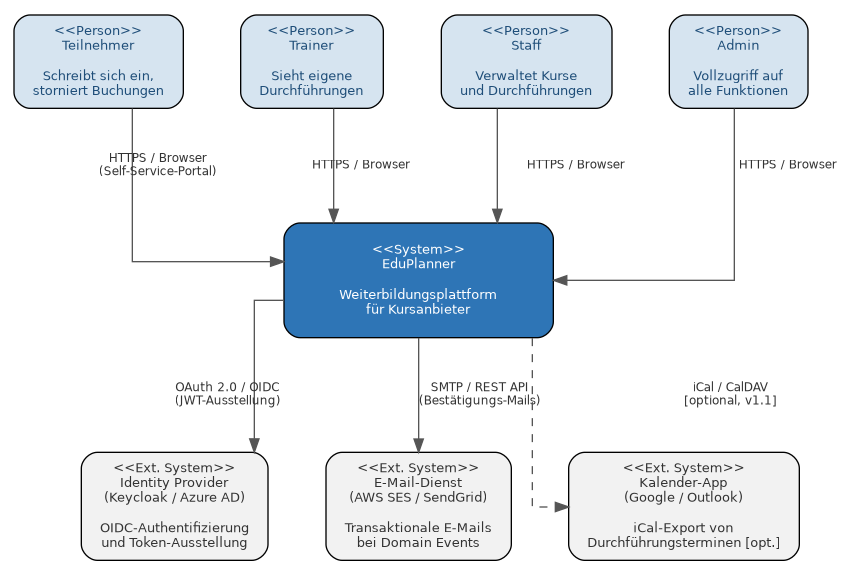
\includegraphics[width=0.95\linewidth]{assets/context_diagram}
  \caption{Grossansicht -- \textit{C4-Kontextdiagramm EduPlanner}
    (vgl.\ Kap.~3.1, Abb.~\ref{fig:context_diagram})}
\end{figure}
\end{landscape}

% ── DDD Context Map ─────────────────────────────────────────
\begin{landscape}
\begin{figure}[p]
  \centering
  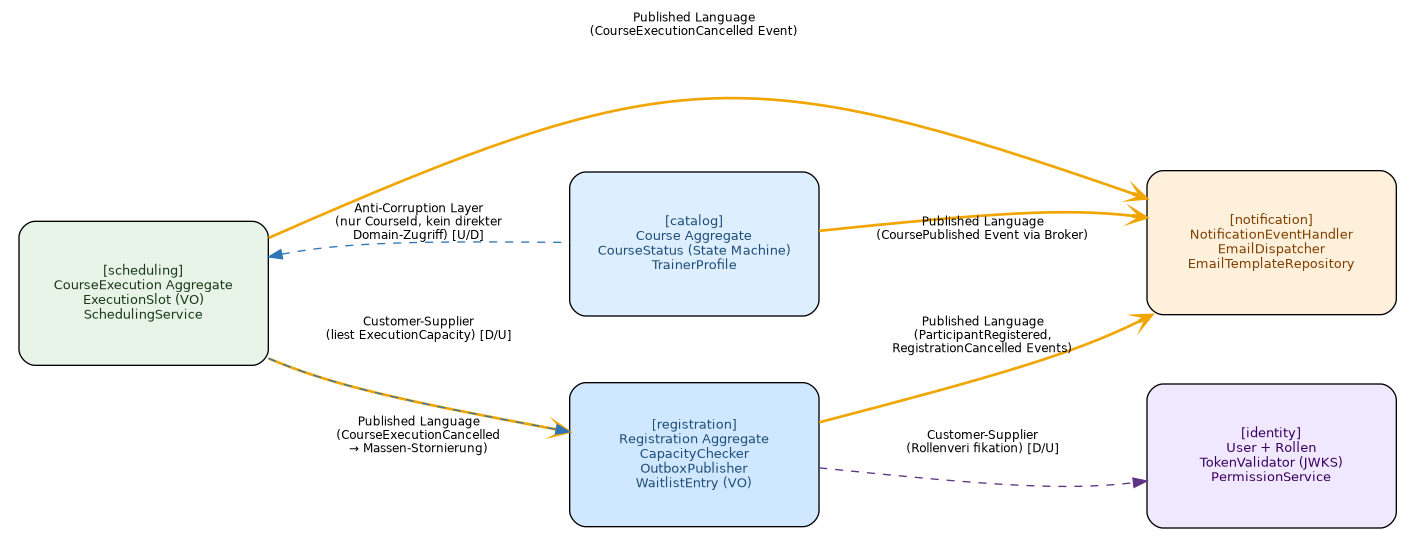
\includegraphics[width=0.95\linewidth]{assets/context_map}
  \caption{Grossansicht -- \textit{DDD Context Map: Bounded Contexts und Beziehungen}
    (vgl.\ Kap.~4.2.2, Abb.~\ref{fig:context_map})}
\end{figure}
\end{landscape}

% ── C4 Container Diagramm (Ebene 1) ─────────────────────────
\begin{landscape}
\begin{figure}[p]
  \centering
  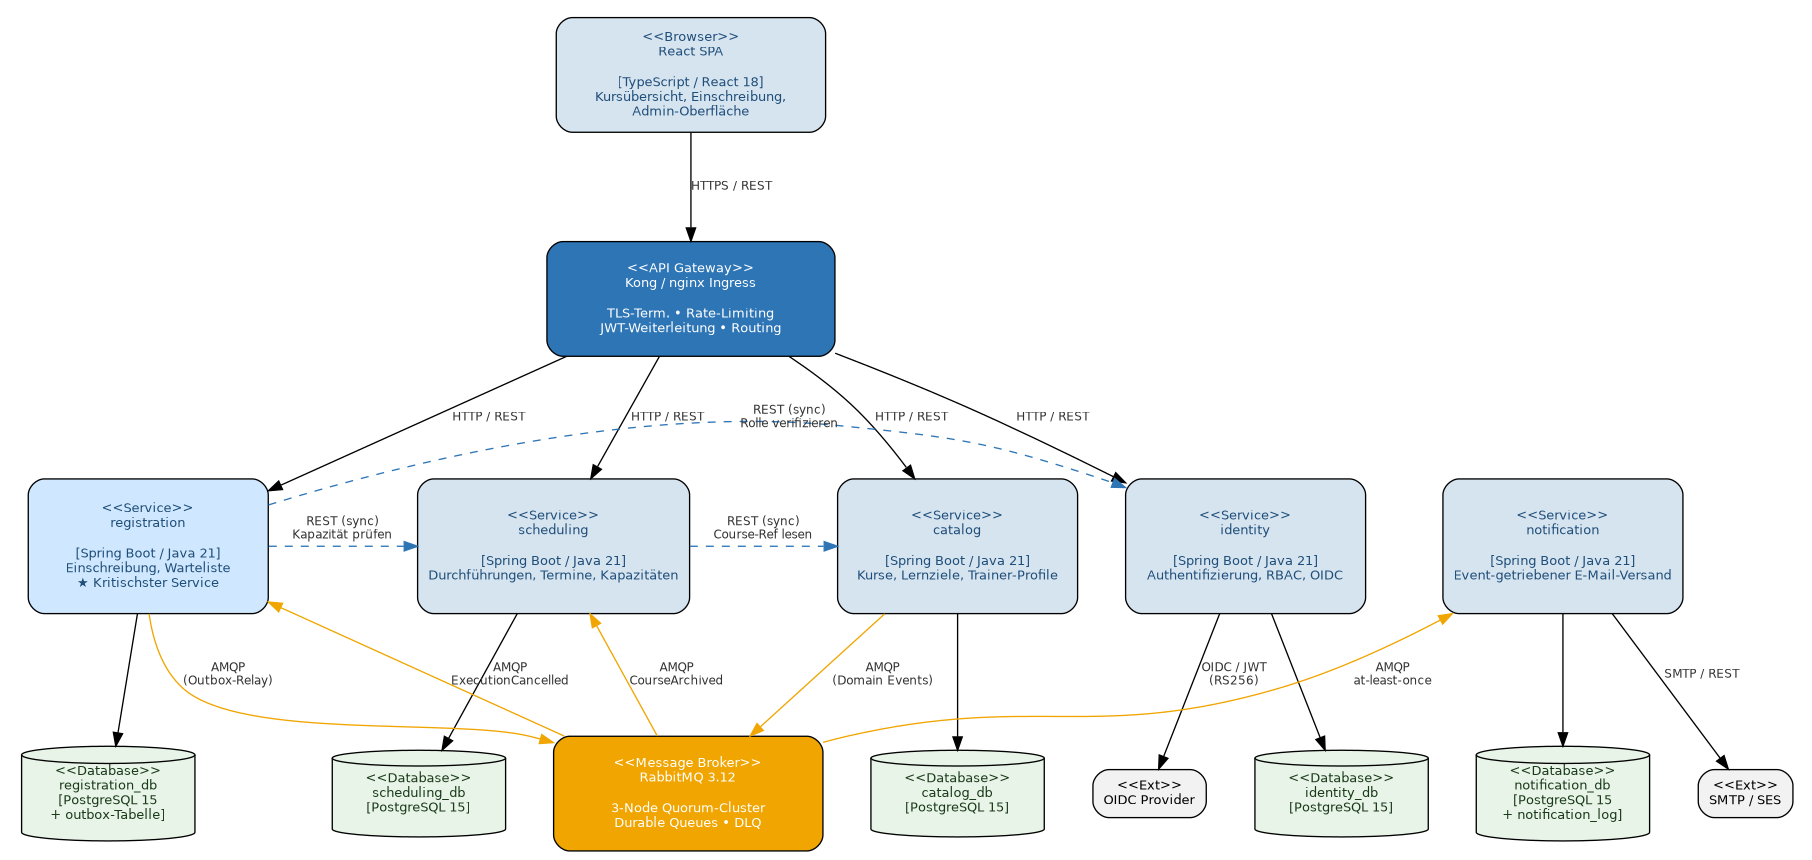
\includegraphics[width=0.95\linewidth]{assets/ebene1_container_diagram}
  \caption{Grossansicht -- \textit{C4-Container-Diagramm: Gesamtsystem EduPlanner}
    (vgl.\ Kap.~5.1, Abb.~\ref{fig:container})}
\end{figure}
\end{landscape}

% ── catalog Service ──────────────────────────────────────────
\begin{landscape}
\begin{figure}[p]
  \centering
  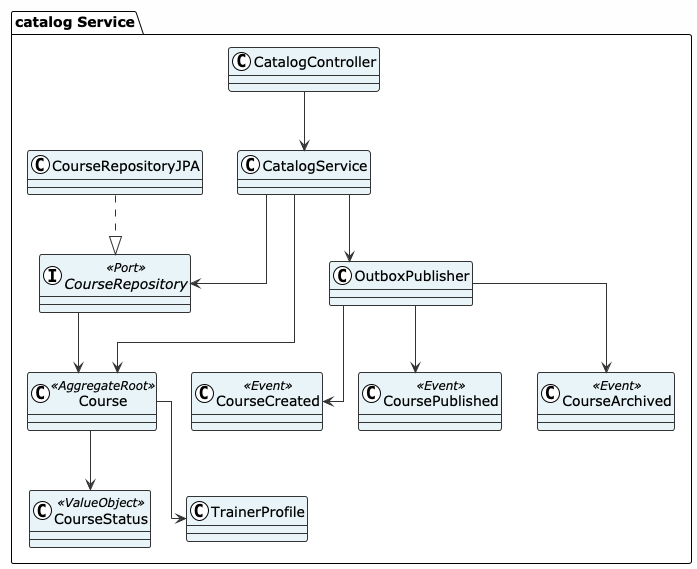
\includegraphics[width=0.85\linewidth]{assets/ebene2_catalog_class_diagram}
  \caption{Grossansicht -- \textit{UML-Klassendiagramm: \texttt{catalog}-Service}
    (vgl.\ Kap.~5.2, Abb.~\ref{fig:catalog})}
\end{figure}
\end{landscape}

% ── CourseStatus Zustandsdiagramm ───────────────────────────
\begin{landscape}
\begin{figure}[p]
  \centering
  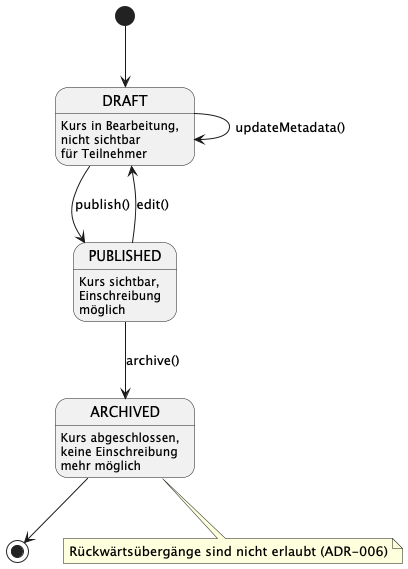
\includegraphics[width=0.70\linewidth]{assets/catalog_course_state_machine}
  \caption{Grossansicht -- \textit{Zustandsübergangsdiagramm \texttt{CourseStatus}}
    (vgl.\ Kap.~5.2.1, Abb.~\ref{fig:course-state})}
\end{figure}
\end{landscape}

% ── scheduling Service ───────────────────────────────────────
\begin{landscape}
\begin{figure}[p]
  \centering
  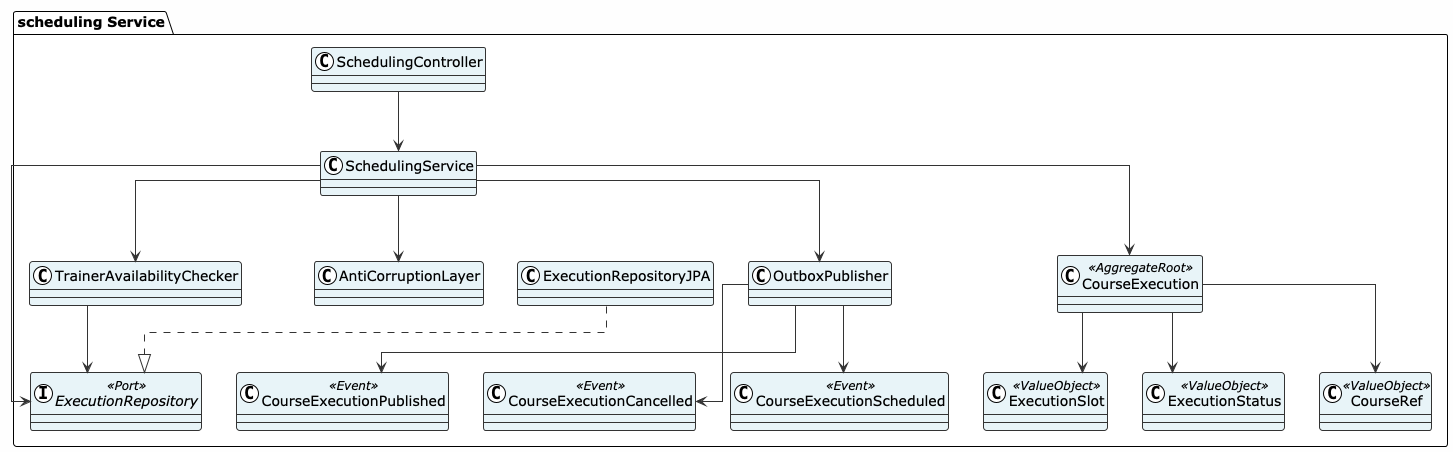
\includegraphics[width=0.95\linewidth]{assets/ebene2_scheduling_class_diagram}
  \caption{Grossansicht -- \textit{UML-Klassendiagramm: \texttt{scheduling}-Service
    inkl.\ Anti-Corruption Layer}
    (vgl.\ Kap.~5.3, Abb.~\ref{fig:scheduling})}
\end{figure}
\end{landscape}

% ── registration Service ─────────────────────────────────────
\begin{landscape}
\begin{figure}[p]
  \centering
  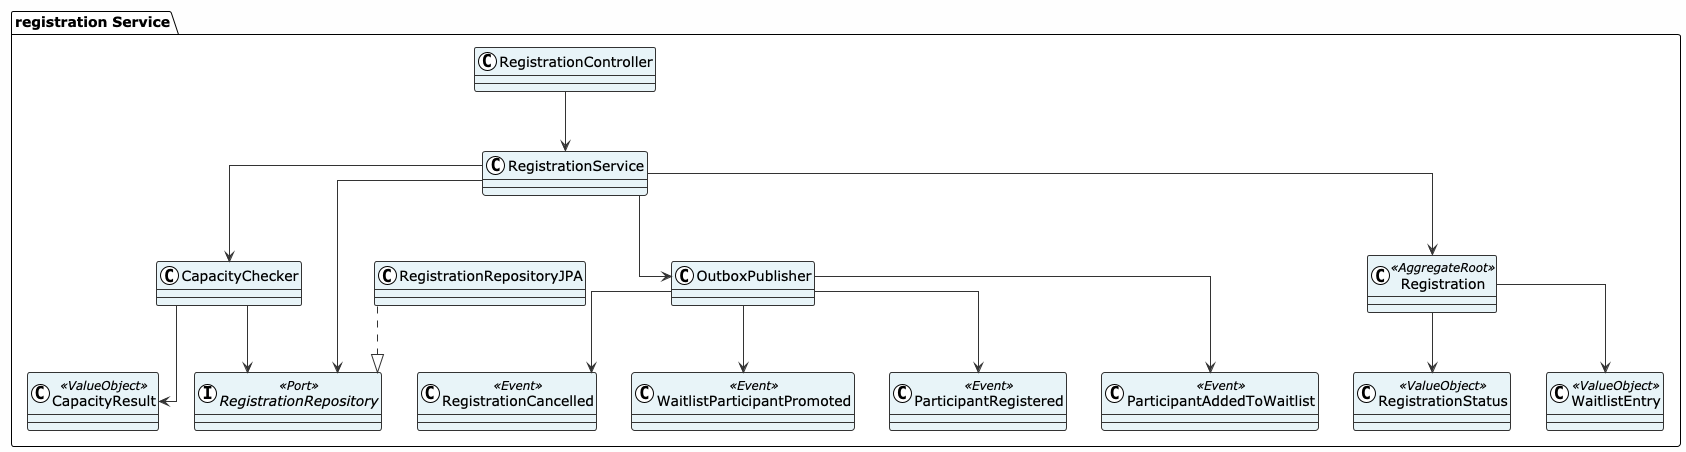
\includegraphics[width=0.95\linewidth]{assets/ebene2_registration_class_diagram}
  \caption{Grossansicht -- \textit{UML-Klassendiagramm: \texttt{registration}-Service}
    (vgl.\ Kap.~5.4, Abb.~\ref{fig:registration})}
\end{figure}
\end{landscape}

% ── notification Service ─────────────────────────────────────
\begin{landscape}
\begin{figure}[p]
  \centering
  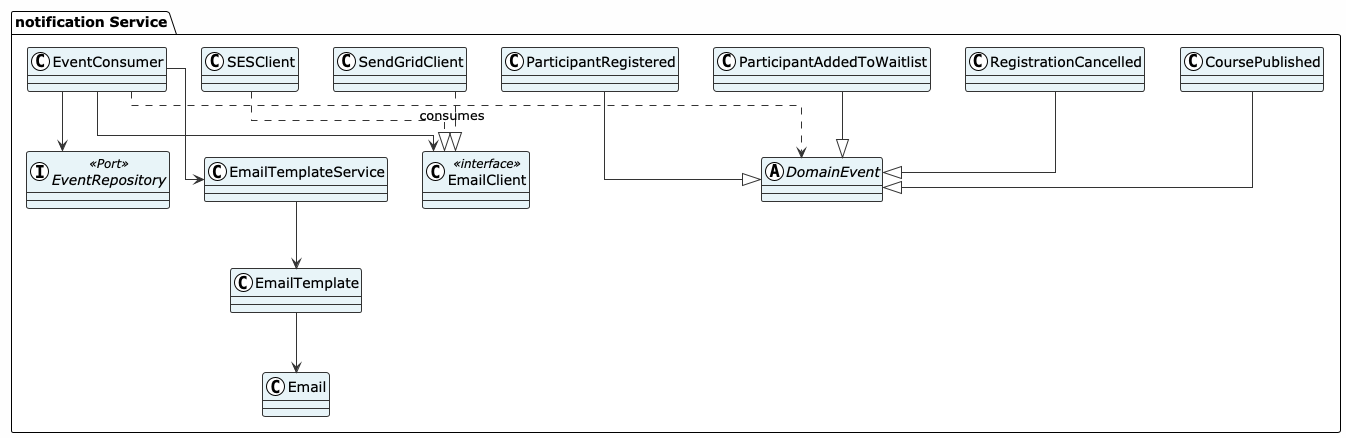
\includegraphics[width=0.85\linewidth]{assets/ebene2_notification_class_diagram}
  \caption{Grossansicht -- \textit{UML-Klassendiagramm: \texttt{notification}-Service}
    (vgl.\ Kap.~5.5, Abb.~\ref{fig:notification})}
\end{figure}
\end{landscape}

% ── identity Service ─────────────────────────────────────────
\begin{landscape}
\begin{figure}[p]
  \centering
  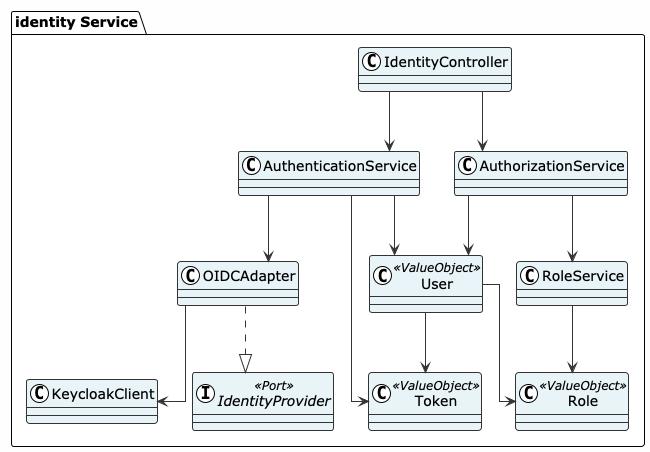
\includegraphics[width=0.85\linewidth]{assets/ebene2_identity_class_diagram}
  \caption{Grossansicht -- \textit{UML-Klassendiagramm: \texttt{identity}-Service}
    (vgl.\ Kap.~5.6, Abb.~\ref{fig:identity})}
\end{figure}
\end{landscape}

% ── Sequenzdiagramm 1 ────────────────────────────────────────
\begin{landscape}
\begin{figure}[p]
  \centering
  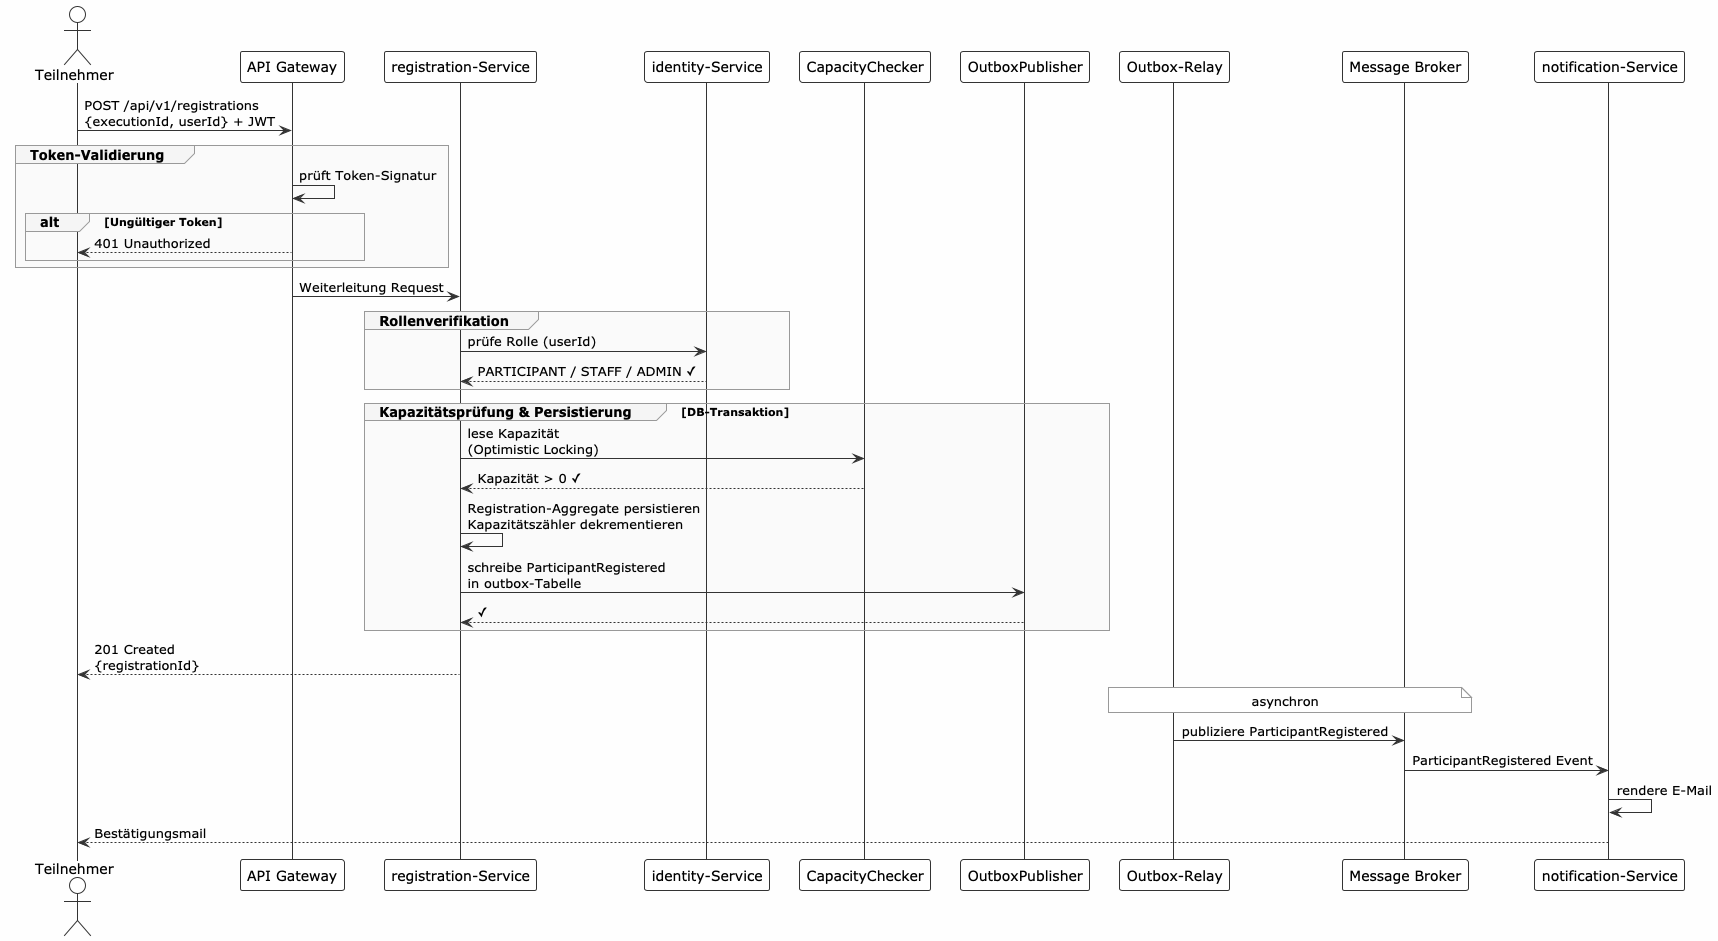
\includegraphics[width=0.95\linewidth]{assets/sequence_diagram_1}
  \caption{Grossansicht -- \textit{Szenario~1: Teilnehmer schreibt sich ein (Happy Path)}
    (vgl.\ Kap.~6.1, Abb.~\ref{fig:sequence_diagram_1})}
\end{figure}
\end{landscape}

% ── Sequenzdiagramm 2 ────────────────────────────────────────
\begin{landscape}
\begin{figure}[p]
  \centering
  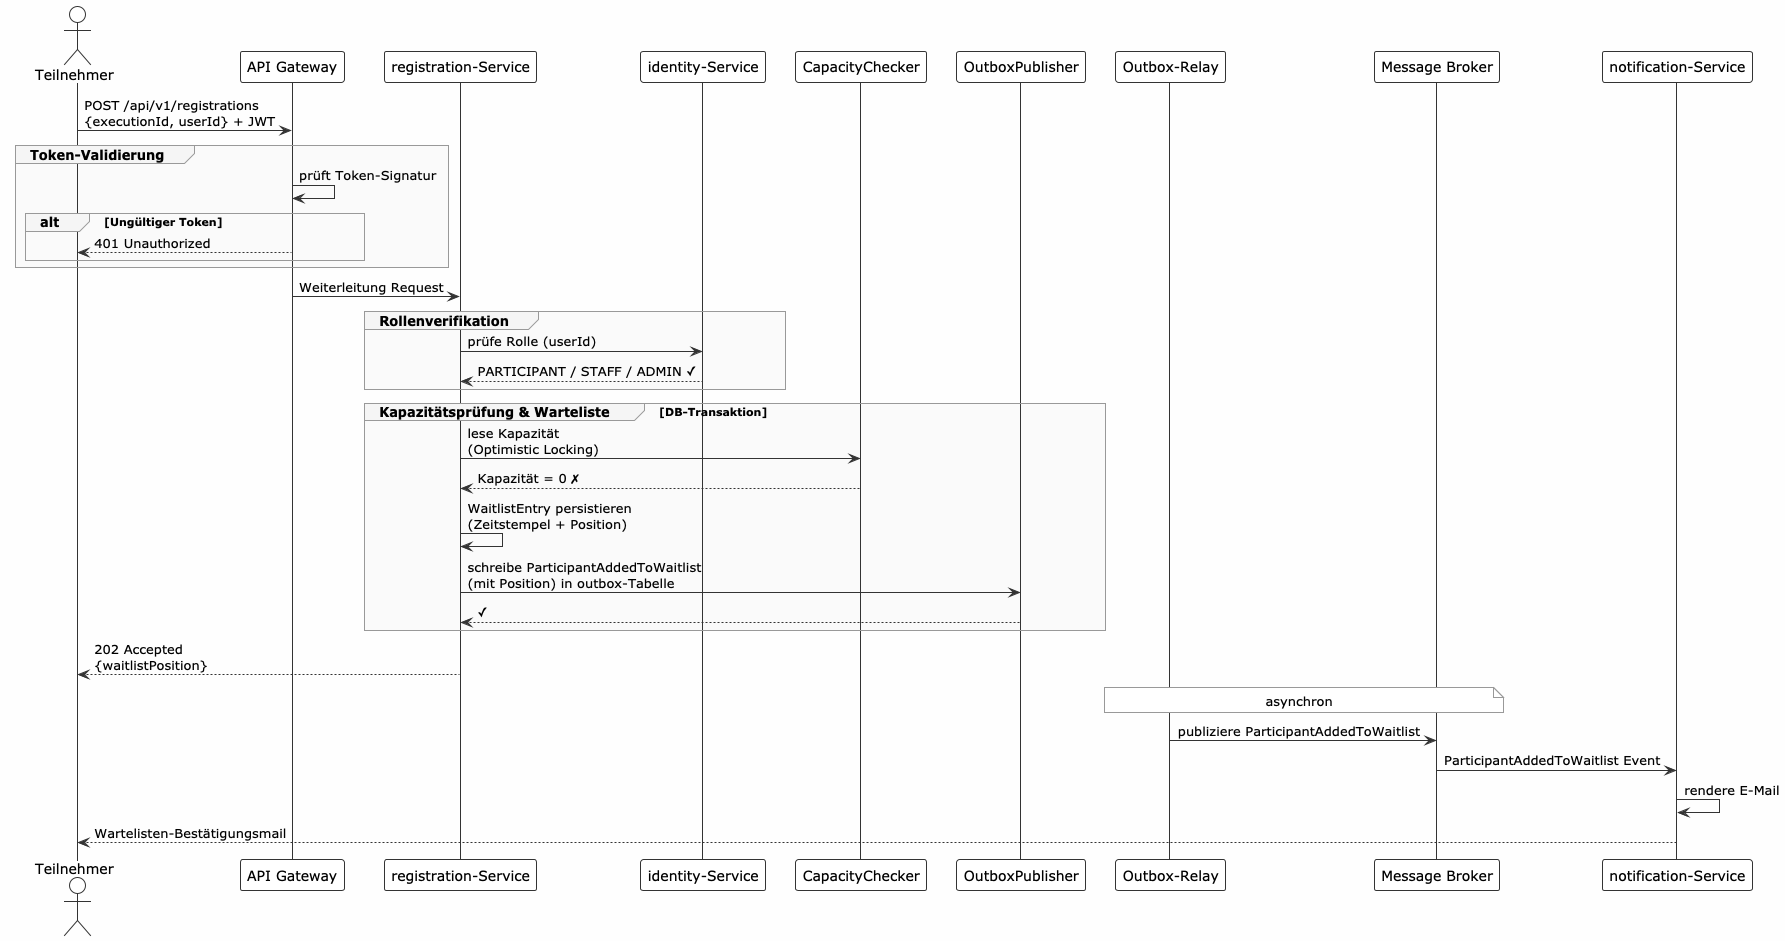
\includegraphics[width=0.95\linewidth]{assets/sequence_diagram_2}
  \caption{Grossansicht -- \textit{Szenario~2: Kurs ausgebucht -- Warteliste}
    (vgl.\ Kap.~6.2, Abb.~\ref{fig:sequence_diagram_2})}
\end{figure}
\end{landscape}

% ── Sequenzdiagramm 3 ────────────────────────────────────────
\begin{landscape}
\begin{figure}[p]
  \centering
  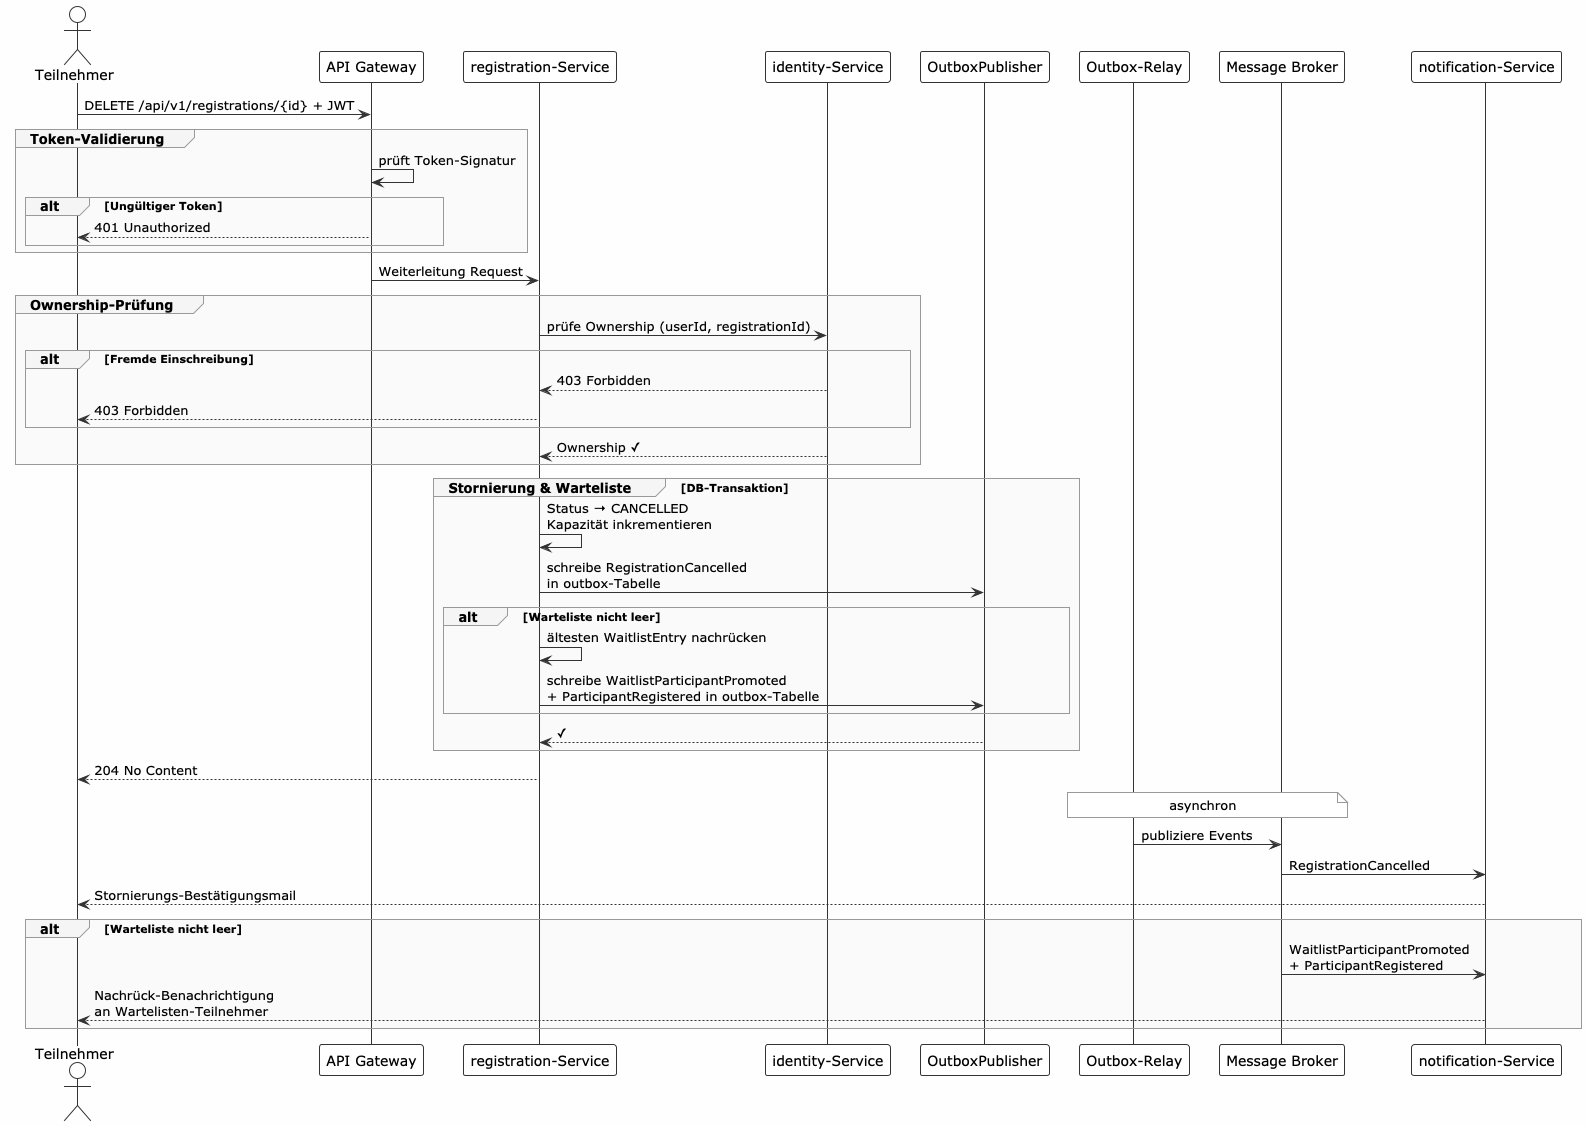
\includegraphics[width=0.95\linewidth]{assets/sequence_diagram_3}
  \caption{Grossansicht -- \textit{Szenario~3: Einschreibung stornieren}
    (vgl.\ Kap.~6.3, Abb.~\ref{fig:sequence_diagram_3})}
\end{figure}
\end{landscape}

% ── Sequenzdiagramm 4 ────────────────────────────────────────
\begin{landscape}
\begin{figure}[p]
  \centering
  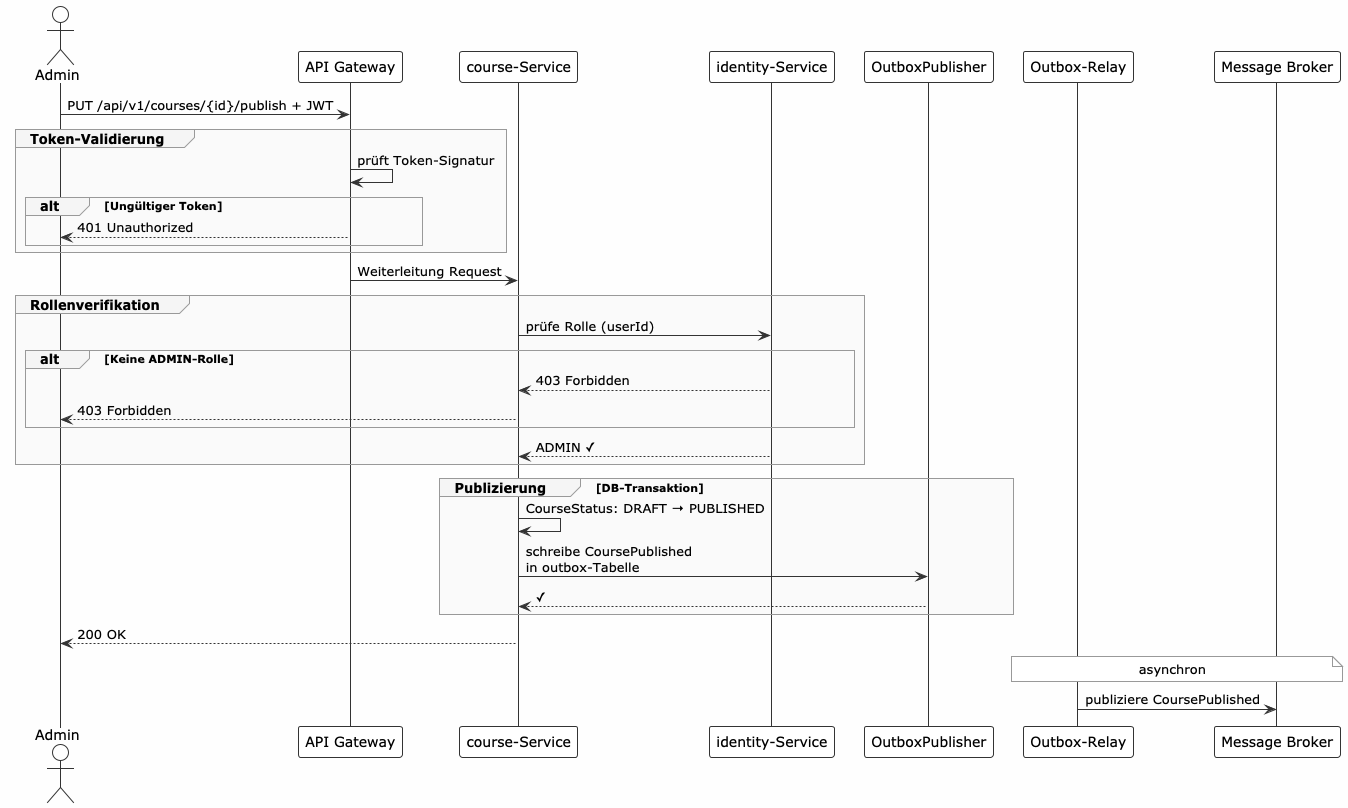
\includegraphics[width=0.95\linewidth]{assets/sequence_diagram_4}
  \caption{Grossansicht -- \textit{Szenario~4: Admin veröffentlicht einen Kurs}
    (vgl.\ Kap.~6.4, Abb.~\ref{fig:sequence_diagram_4})}
\end{figure}
\end{landscape}

% ── Sequenzdiagramm 5 ────────────────────────────────────────
\begin{landscape}
\begin{figure}[p]
  \centering
  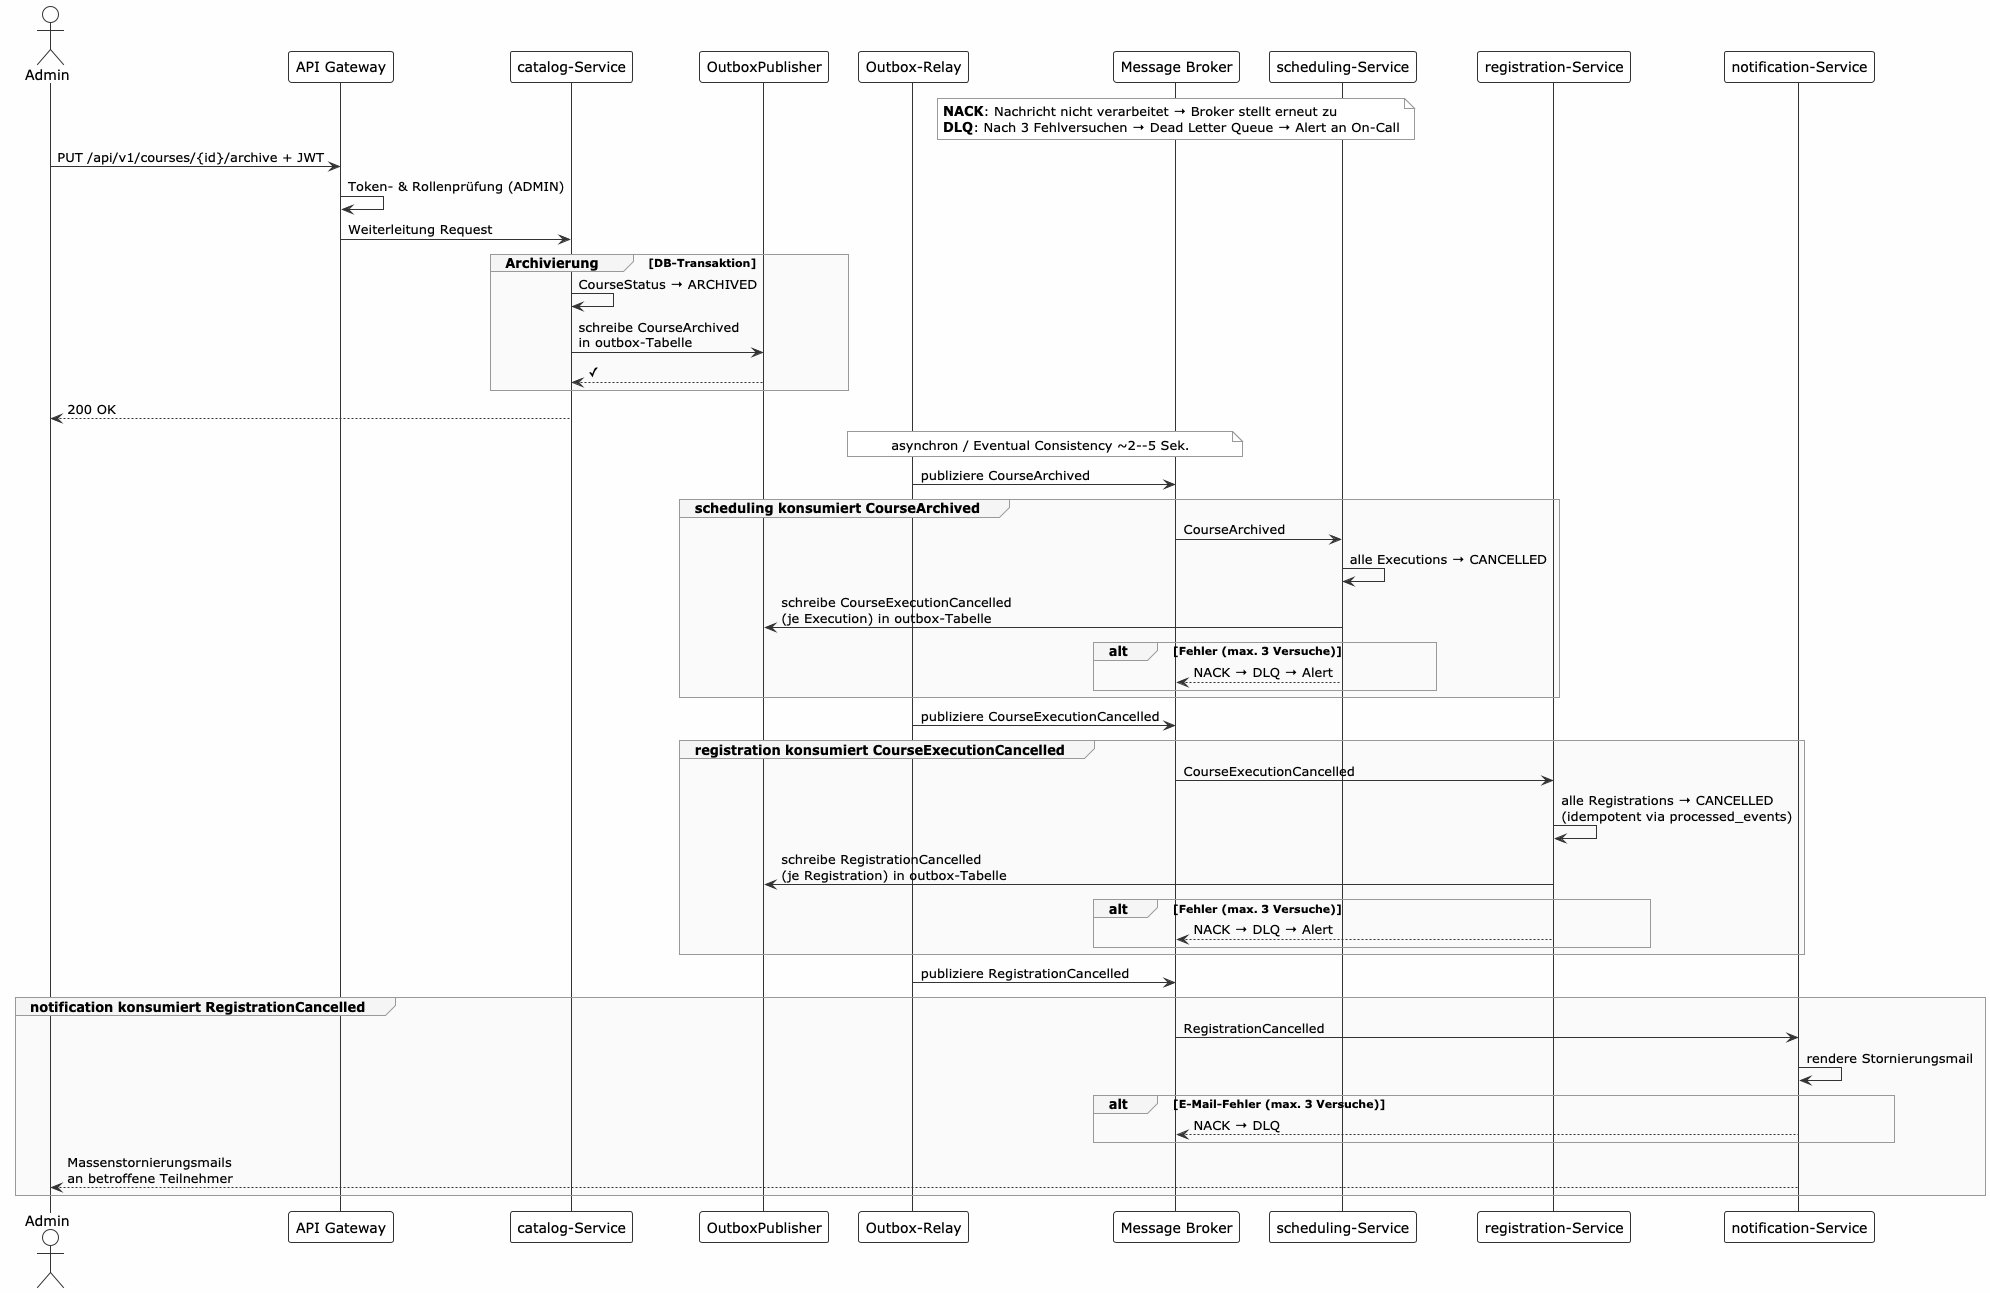
\includegraphics[width=0.95\linewidth]{assets/sequence_diagram_5}
  \caption{Grossansicht -- \textit{Szenario~5: Cross-Context-Transaktion (Kurs archivieren)}
    (vgl.\ Kap.~6.5, Abb.~\ref{fig:sequence_diagram_5})}
\end{figure}
\end{landscape}

% ── Deployment-Diagramm ──────────────────────────────────────
\begin{landscape}
\begin{figure}[p]
  \centering
  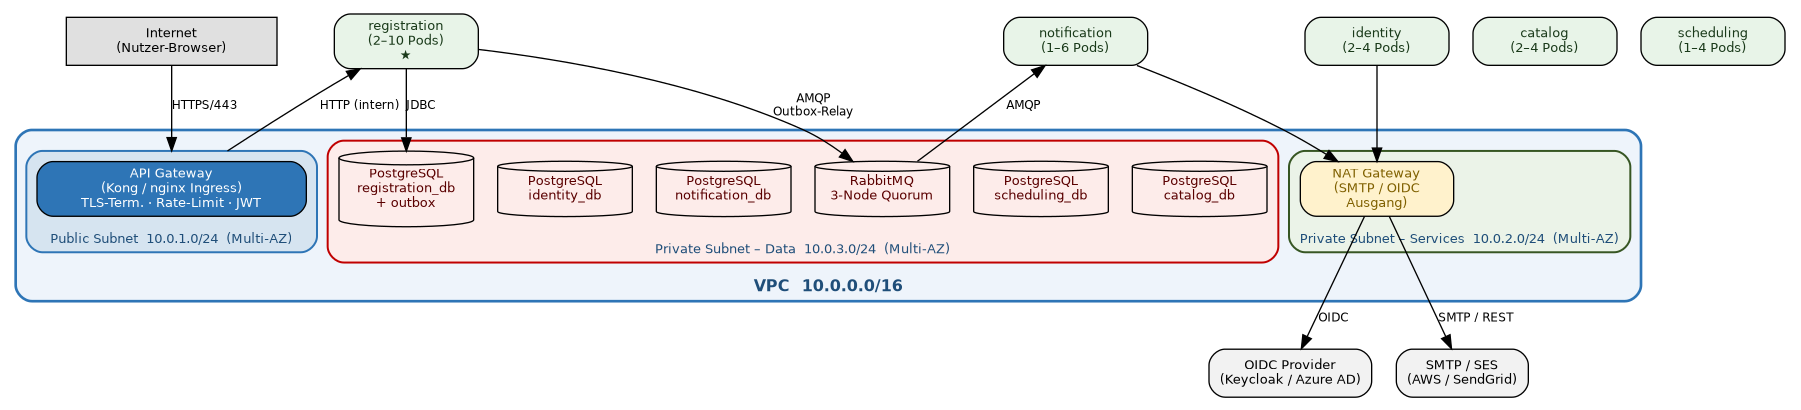
\includegraphics[width=0.95\linewidth]{assets/deployment_diagram}
  \caption{Grossansicht -- \textit{Deployment-Diagramm: Netzwerk-Topologie Kubernetes / Azure}
    (vgl.\ Kap.~7.1, Abb.~\ref{fig:deployment_diagram})}
\end{figure}
\end{landscape}

% ── Qualitätsbaum ────────────────────────────────────────────
\begin{landscape}
\begin{figure}[p]
  \centering
  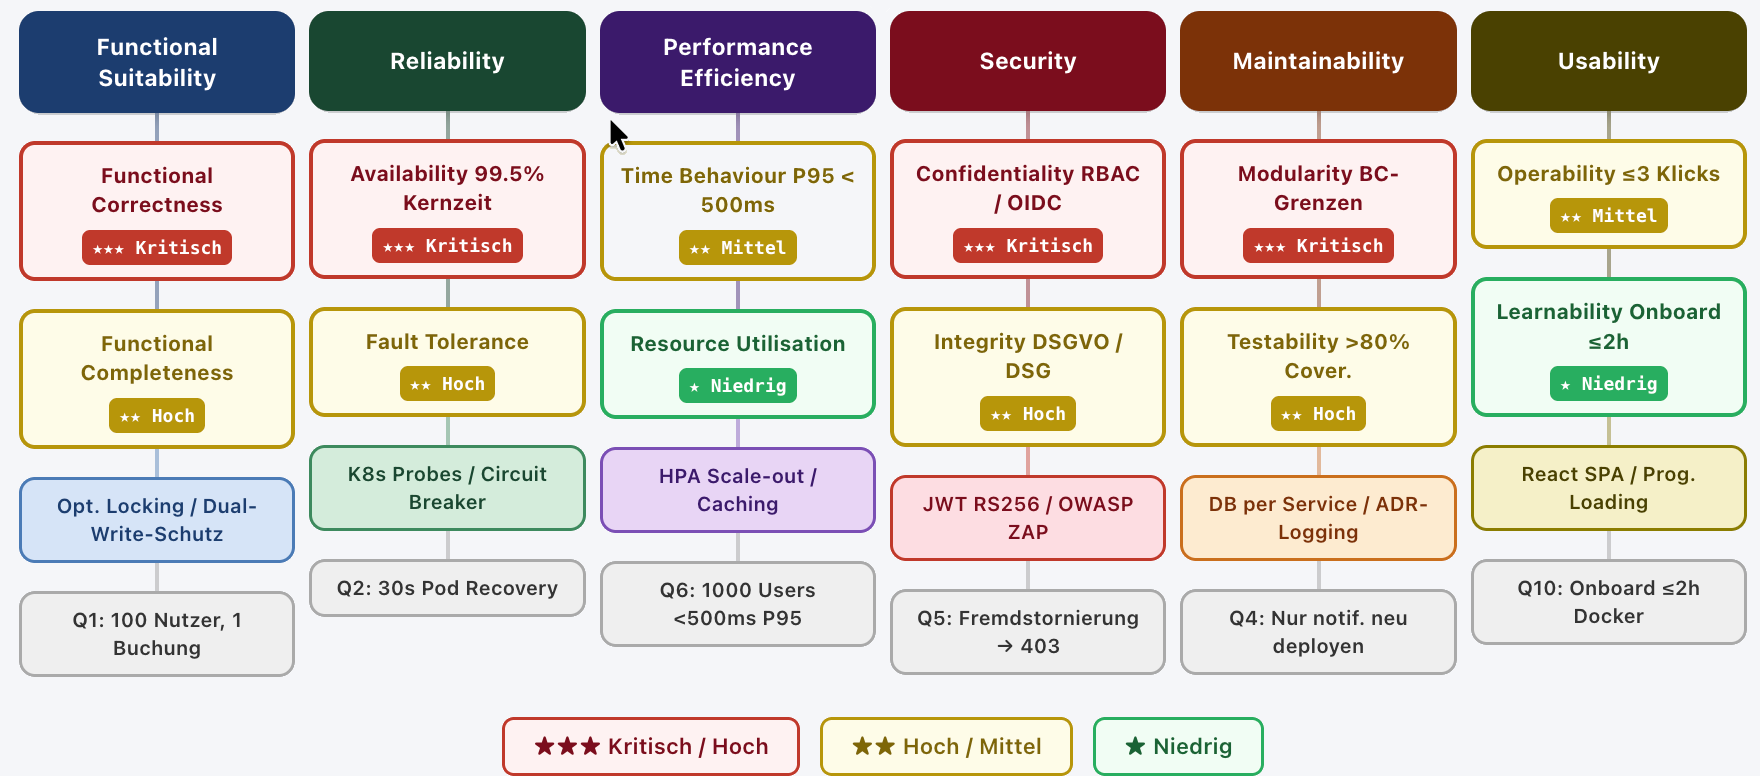
\includegraphics[width=0.95\linewidth]{assets/QualityTree}
  \caption{Grossansicht -- \textit{Qualitätsbaum: EduPlanner Qualitätsanforderungen}
    (vgl.\ Kap.~10.1, Abb.~\ref{fig:QualityTree})}
\end{figure}
\end{landscape}

% ── Risikobewertungsmatrix ───────────────────────────────────
\begin{landscape}
\begin{figure}[p]
  \centering
  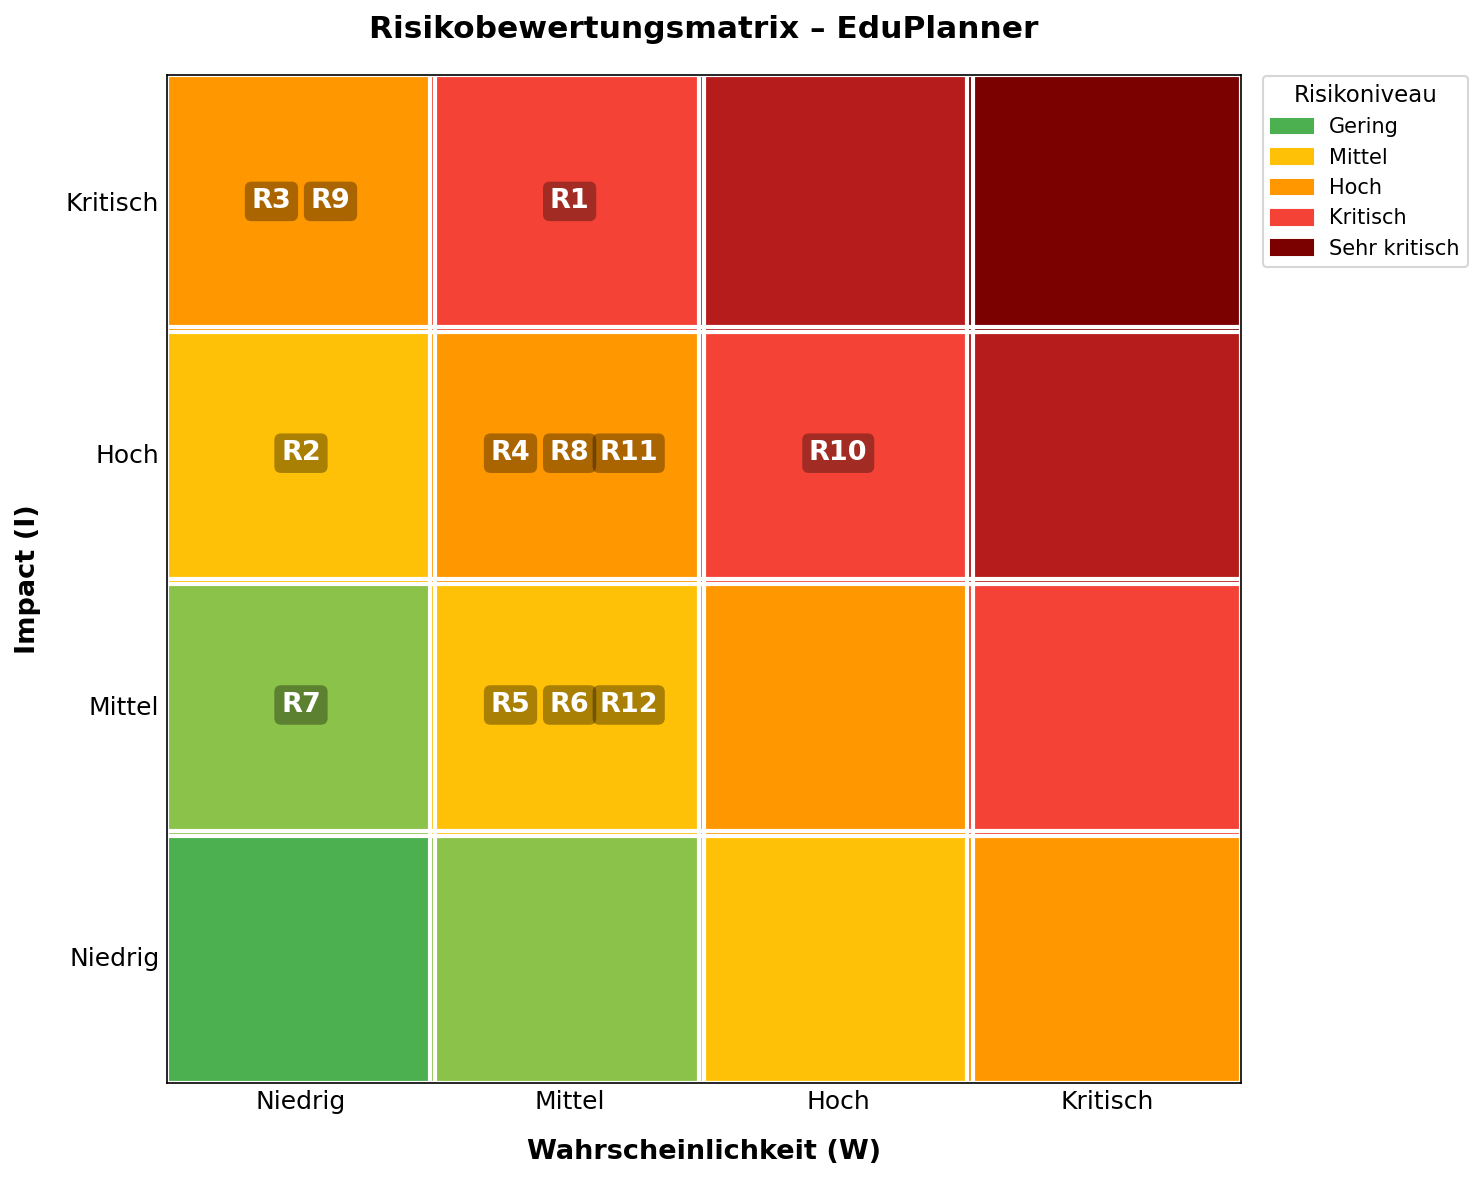
\includegraphics[width=0.85\linewidth]{assets/RiskMatrix}
  \caption{Grossansicht -- \textit{Risikobewertungsmatrix: Wahrscheinlichkeit vs.\ Impact (R1--R12)}
    (vgl.\ Kap.~11.1, Abb.~\ref{fig:RiskMatrix})}
\end{figure}
\end{landscape}
